\chapter{Foundation}
\label{sec:foundation}

Before dealing with the problem setup of the Master Thesis itself, in the following chapter, a broad foundation
of graphs and Graph Learning will be given. Moreover, some important mathematically concepts and methods will be introduced as well as cryo-EM.
%A more detailed explanation to some sections will follow in the Section~\nameref{sec:relatedWork}

\section{Graph Foundations}
A graph is defined as  $G = \langle V,E \rangle$, where $V$ is a set of 
vertices (or nodes) and $E$ is a set of edges (or links). 
Edges are defined as a set of tuples $\langle i,j \rangle$, where $i$ and $j$ determine the 
index of the vertices in the graph.

Edges of the graph can be either \textit{directed} or \textit{undirected} and has to do with the position of the 
nodes in the edge. In a directed graph, a edge points explicitly from
one node to another, which means that edge $\langle i,j \rangle \neq \langle j,i \rangle$. 
In undirected graphs the ordering does not matter and $\langle i,j \rangle = \langle j,i \rangle$.

Moreover, edges can have weights, which is a method to define some kind of importance to the neighbours of a node.
If edges are dealing with weights, we are talking from a \textit{weighted} graph.

A \textit{dense} graph is a graph, where the number of edges is close to the maximal number of edges.
Contrarily, a \textit{sparse} graph only consists of a few edges.

\textit{Homophilic} and \textit{heterophilic} are properties of the graph and are from importance in link predication. 
A homophilic dataset leads to the tendency to interact with similar nodes, therefore nodes will be linked with a edge. 
Whereas a heterophilic dataset contrary has the tendency to not link, if nodes are similar.

\subsection{Important matrices}
To do calculation with graphs, it is common to translate graphs in a well suitable mathematically
form, which are matrices. In the following, some important matrices will be introduced.

\paragraph{Adjacency matrix:}

The (binary) adjacency matrix of graph $G$ is defined as follows:
\begin{equation}
    \label{eg:AdjacencyMatrix}
    A_{ij} =    
    \begin{cases}
        %1  & \text{if } \norm{\biggl y_i - y_j \biggr} < \tau\\
        1  & \text{if } \langle i , j \rangle \in E \\
        0, & \text{otherwise}
    \end{cases}
\end{equation}

The matrix $A$ has dimension $\mathbb{R}^{N \times N}$ and the indices of the matrix correspond to the nodes of the graph.
If there is an edge between two nodes, the entry in the matrix will be set to $1$, otherwise to $0$.
This leads to an unweighted graph, as the weight of all edges will be $1$. 

When the graph is undirected, the resulting matrix will be symmetric and has a complete set of eigenvalues
and eigenvectors. The set of eigenvalues are also called \textit{spectrum} of the graph.

\subparagraph{K-hop neighbourhood:}
The adjacency matrix $A$ has many nice properties, and one is referred to the k-hop neighbourhood. 
When calculating the $k$-th power of $A$, on calculates the k-hop neighbourhood of the graph.
The resulting matrix gives the number of walks of length $k$ from one node to another.
Moreover, with $A[i]$, one can determine the k-hop neighbourhood of node $i$. 
Every node in the extracted row, which has a value $> 0$ can be reached within $k$ hops.

\paragraph{Degree matrix:}
The degree matrix of $G$ is defined as follows:
\begin{equation}
    D_{ij} =    
    \begin{cases}
        %1  & \text{if } \norm{\biggl y_i - y_j \biggr} < \tau\\
        deg(v_i)  & \text{if } i = j \\
        0, & \text{otherwise}
    \end{cases}
\end{equation}

Where $deg(v_i)$ is the degree of the node, formally the number of incoming edges of node $v_i$.

\paragraph{Normalization:}
When starting calculating with matrix A, it is sometimes necessary to normalize.
With the degree matrix $D$ and adjacency matrix $A$, all information for normalization are present.
The normalization can be achieved in a row, column or symmetric way:
\begin{equation}
    \begin{aligned}
        A_{row-norm} &= D^{-1} A
        A_{col-norm} &= A D^{-1}
        A_{sym}      &=  D^{-\frac{1}{2}} A D^{-\frac{1}{2}}    
    \end{aligned}
\end{equation}

The normalization of the row and column will normalize the row and column to sum to $1$ respectively.
The symmetric normalization is well suited for undirected graphs, as it preserve the nice symmetric structure matrices.


\paragraph{Graph Laplacian}
The graph Laplacian is a matrix that represents the graph and can be used to find many important properties of the graph. 
It is defined as follows:
\begin{equation}
    L = D - A
\end{equation}

\paragraph{Normalized Graph Laplacian:}
During computation, it is often needed to have a normalized version of the Graph Laplacian: \newline
\begin{equation}
    \begin{aligned}
        L_{sym} &= I - D^{-\frac{1}{2}} A D^{-\frac{1}{2}}
        L_{rw}  &= I - D^{-1} A,
    \end{aligned}
\end{equation}
where $L_{sym}$ is a symmetric normalization and $L_{rw}$ is called a random walk normalization.

%\subsubsection{Normalized Graph Laplacian eigen decomposition}
%
%\begin{equation}
%    \begin{aligned}
%        L_{sym} &= U \Lambda U^T \\
%        U &= [u_0, \dots, u_{N-1}] \in R^{N \times N}\\
%        \Lambda &= diag \left ( [\lambda_0, \dots, \lambda_{N-1}]  \right ) \in R^{N \times N}
%    \end{aligned}
%\end{equation}
%
%In this scenario, eigenvectors are also known as \textit{graph Fourier modes}
%and eigenvalues are known as the \textit{spectral frequencies}.
%
%Moreover, with the Graph Fourier Transform, we can calculate these values from a symmetric
%graph Laplacian.

\subsection{Graph Construction}

When data is not available as a graph, it can be constructed from the data.
First of all, every sample can be seen as a node and only the decision of how edges will be constructed
is necessary. One popular approach is k-nearest neighbour (KNN) graph construction. The parameter $k$
defines how many edges every node will have at the end. The neighbourhood of node $i$ is defined
as $\mathcal{N}_i$ and consists of the nodes, with the $k$ smallest similarity measure.

\begin{equation}
    \label{eg:knn}
    A_{ij} =    
    \begin{cases}
        %1  & \text{if } \norm{\biggl y_i - y_j \biggr} < \tau\\
        1  & \text{if } j \in \mathcal{N}_i \\
        0, & \text{otherwise}
    \end{cases}
\end{equation}

Instead of using a fixed parameter $k$ as in KNN approach, one could define a threshold $\pi$
and connection nodes if the similarity measure is smaller than $\pi$. This is another common way
to define graphs and results in a graph, where not all nodes have the same amount of edges.

\section{Graph Denoising}
Data acquired by Real-world observations are often noisy, which can lead to poor 
performance on data analysis tasks. This observed data can already be in the form of a graph,
or a graph can be easily constructed. This resulting graph is what we call
a noisy graph, as it includes the noise from the observation.

Graph denoising is the task to reconstruct the original graph from a noisy one.
Therefore, graph denoising can be seen as a pre-processing step, where noisy data is filtered.

Denoising in general has often to do with averaging 
 and graphs are a well suited data structure for this task\cite{noneLocalMean}.

\paragraph{Noise:}
A noisy observation is defined as:
$y_n = y + \eta$, where $\eta$ is the observation noise and $y$ the noiseless observation.

\paragraph{Denoising:}
When we talk from denoising, we want to reconstruct the true observation 
from a given noisy observation. 
This reconstruction is done via averaging, which can be performed
locally, by the calculus of variations or in the frequency domain\cite{noneLocalMean}.

\paragraph{Noisy Graph}:
For every noisy graph, there exists an original graph $G = \langle V,E \rangle$.

The noisy graph can be defined as follows:
\begin{equation}
    \begin{aligned}
        G_{noisy} &= \langle V,E_{noisy} \rangle,  \\ 
        \text{ with }  E_{noisy} &= E \setminus  E^{-} \cup  E^{+}, \\ 
         E^{-} & \subseteq E, \\
         E^{+} \cap E &= \emptyset
    \end{aligned}
\end{equation}

The noisy graph consists of the same vertices as the original graph. From
the original graphs edges, some are removed (denoted by $E^{-}$) and some new edges are added
(denoted by $E^{+}$).

The adjacency matrix of $G_{noisy}$ is denoted by $\bar{A}_{ij}$.
The task of graph denoising, can therefore be written as:
\begin{equation}
    \bar{A} \xrightarrow[method]{Graph-denoising} \tilde{A} \approx A
\end{equation}

Where $\bar{A}$, $\tilde{A}$, $A$ denotes the adjacency matrix from the noisy input graph, the denoised
 graph and the original graph respectively.

\subparagraph{Connection to link prediction}
Link prediction is a task in Graph Learning. 
The idea is to predict existence of a link (edge) between two nodes.
The task can be formulated as a missing value estimation task. A model $M_p$ is learned
from a given set of observed edges. The model finally maps links to probabilities:


\begin{equation}
    M_p : E^{\prime} \rightarrow [0,1],
\end{equation}

where $E^{\prime}$ is the set of potential links.

We define $U$ as the set of all possible vertices of $G$, therefore $E \subseteq U$.
Obviously, graph denoising can be seen as a link prediction problem.

The difference is, that in link prediction a model from a set of observed links is learned
$E_{observed} \subseteq E$ and in graph denoising the model is learned from 
$E_{observed} \subseteq U$. 

On could also say that link prediction problems are a subset of graph denoising problems.


\section{Math Foundation}
In the following section, some mathematically concepts and methods will be explained.

\subsection{Embedding}
Mathematically, an embedding $f: X \rightarrow Y$ is defined as a structure-preserving mapping from one domain to another.

In graph theory, a graph embedding in the mapping from the graph $G$ to a surface structure $\Sigma$. 


\subsection{Manifolds}
A manifold is a topological space, where locally Euclidean distances make sense.
More formally, a $n$-dimensional manifold is a topological space where
each point has e neighbourhood, that is homeomorphic (mapping which preserves topological properties) to an subset of a n-dimensional
Euclidean space.

Some example for a 1-D manifold is a line or a circle. 2-D manifolds can already become 
pretty complex and are basically any surfaces like planes, sphere but also the torus,
Klein bottle or others.

\paragraph{Manifold assumption:}
\label{sec:manifoldAssumption}

The manifold assumption is a popular assumption for high-dimensional datasets.
Even if a given dataset is in high-dimension and consists of many features, one can assume,
that these data points are samples from a low-dimensional manifold, 
which embeds the high-dimensional space.

Therefore, if one can approximate the underlying Manifold, one solved the dimensionality reduction
as one can embed the data points in the low-dimensional manifold space.

There is a complete area of research devoted to this manifold assumption called Manifold Learning\cite{ManifoldLearning}.

\subsection{Power Iterations}
\label{sec:powerIterations}

Power iteration (also called power method) is a iteratively method, 
which approximates the biggest eigenvalue of a diagonalizable matrix $A$.

The algorithm starts with a random vector $b_0$ or an approximation of the dominant eigenvector.

\begin{equation}
    \label{eq:powerIterations}
    b_{k+1} = \frac{Ab_k}{||Ab_k||}
\end{equation}

The algorithm not necessarily converges. The algorithm will converge, if $A$ has an eigenvalue strictly grater than its other eigenvalues
and the initial vector $b_0$ has a component in direction of an eigenvector, associated with the dominant eigenvector.

\subsection{Folded spectrum Method}
\label{sec:FoldedSpectrumMethod}
Calculation of eigenvalues and eigenvectors of a given Hamiltonian matrix $H$ 
is a fundamental mathematical problem. Often, we are interested in just the smallest 
values, which can be efficiently computed. But if we are interested in selected values,
this can be hard. $H$ is needed to be diagonalized (bring matrix $H$ into diagonal form) 
which is computationally expensive and for big matrices impossible.

Currently, the best way to solve such problems is the Folded spectrum (FS)\cite{foldedSpectrumMethod} method,
which iteratively solves the problem. During calculation, the eigenvalue spectrum will be folded around a reference 
value $\epsilon$.

\begin{equation}
    \label{eq:foldedSpectrumMethod}
    v^{t+1} = v^t - \alpha (H - \epsilon I )^2 v^t ,
\end{equation}

with $0 < \alpha < 1$. When $t \rightarrow \infty$, then $v^{\infty}$ will be the 
eigenvector with respect to the reference value $\epsilon$.


\subsection{Wasserstein metric}
\label{sec:wasserstein-metric}
The Wasserstein metric is a distance measure between two probability distributions and it is used in ML as a loss function\cite{learningWithWasserstein}. 
Intuitively, it can can be understood as the minimum cost to transfer the mass of one distribution to the other.
Therefore, it is also known as the \textit{earth mover's distance}.

As \citet{wassersteinGAN} could show, ordinary distance measures like \textit{Total Variation}, \textit{Kullback-Leibler divergence}
and \textit{Jensen-Shannon divergence} are not sensible when learning with distributions supported by manifolds
On the contrary, Wasserstein metric does a good job as loss function in such scenarios.


\subsection{Fourier Transform}
\textit{Fourier Analysis} is the overall field of study, which deals with representing (or approximating) functions as 
sums of trigonometric functions. When the function is defined in such a way, we are talking from the \textit{Fourier Domain}.

\textit{Fourier transform} (FT) is the way of transforming signals to the Fourier Domain, which is popular in ML.
Basically, with the Fourier transform, a signal can be decomposed to a \textit{Fourier series}, which consists of many weighted sinusoids. 

\subsubsection{Fourier-slice theorem}
The Fourier-slice theorem \cite{fourierSliceTheorem} in 3D is defined as follows:

\begin{equation}
    \label{eq:Fourrier-slice}
    F_2 P_2 = S_2 F_3,
\end{equation}

where $F2$ and $F3$ are FTs in 2D and 3D respectively, P2 is a projection operator ($P_2 : 3D \rightarrow 2D$) and $S2$ is the restriction operator.

As pointed out by \cite{cryoEmMath},
the Fourier-slice theorem is the foundation of the reconstruction problem in computerized tomography (CT), which will be explained in section~\ref{sec:reconstructionProblemCT}.
It states, that the 2D FT of the tomographic projection is the same as the 3D FT restricted to a 2D plane through the origin.
Basically, for the CT reconstruction problem, acquiring samples from known viewing directions is the same 
as sampling the 3D Fourier-space. This concept is exploited by the filter BackProjection algorithms, see section~\ref{sec:filterBackProjection}.

\subsection{Radon Transform}
The radon transform\cite{radonTransform} is the main mathematically concept of tomographic reconstruction.

It is an integral transformation of a function $f(x,y)$, which is defined on the plane. In tomographic reconstruction
the function $f$ will be the observed tomographic image.
The radon transform then transforms $f$ to a function $Rf$, which corresponds to the line integral of the line defined by 
the two parameters $\theta$ and $s$, where $\theta$ is a angle and $s$ the distance to the origin.

In Figure~\ref{fig:phantom_theta45} and Figure~\ref{fig:phantom_theta45_s14} on can see two plots of different
values for $\theta$ and $s$, where $f(x,y)$ is the Shepp-Logan phantom. The complete $Rf(\theta=45, s=0)$, 
which is also called \textit{sinogram}, can be see in Figure~\ref{fig:phantom_sinogram}

\begin{figure}[H]
    \centering
    \subbottom[Radon Transform  $R f(\theta=45, s=0)$\label{fig:phantom_theta45}]{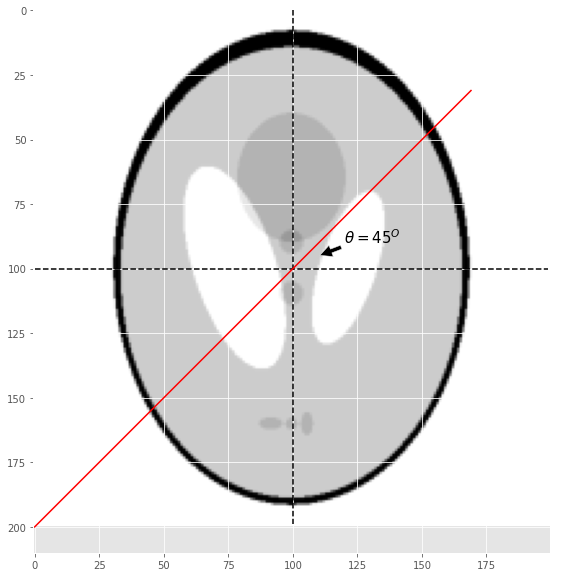
\includegraphics[width=0.3\textwidth]{phantom_theta45.png}}
    \subbottom[Radon Transform  $R f(\theta=45, s=14.14)$\label{fig:phantom_theta45_s14}]{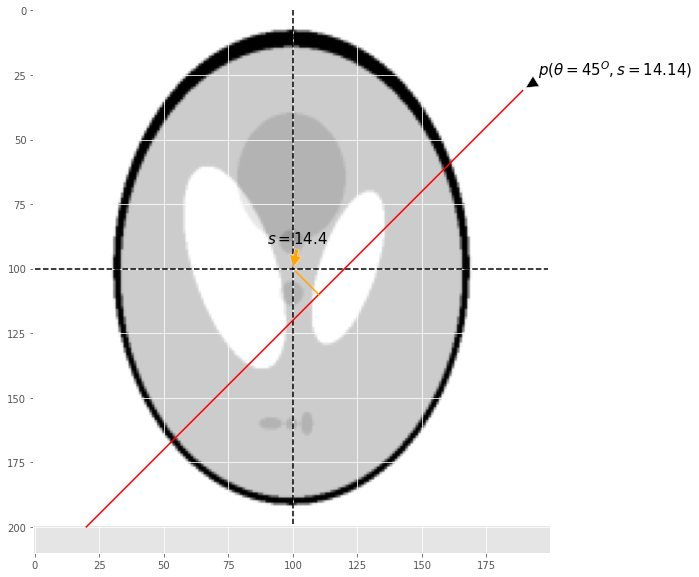
\includegraphics[width=0.3\textwidth]{phantom_theta45_s14.png}}
    \subbottom[Shepp–Logan phantom sinogram of $Rf(\theta=45, s=0)$\label{fig:phantom_sinogram}]{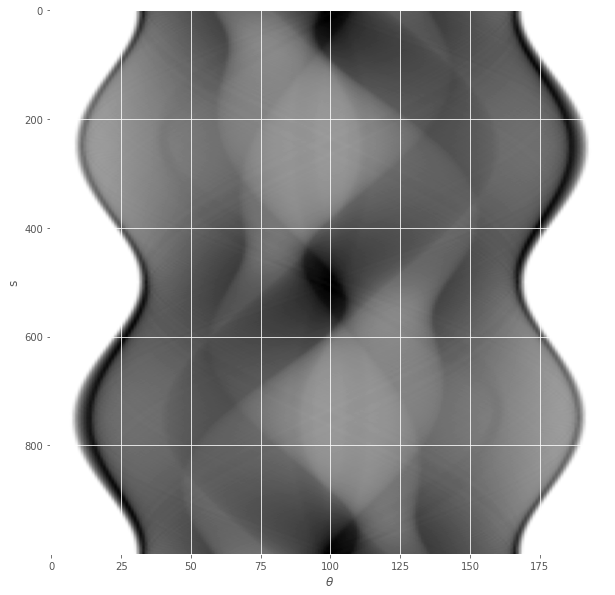
\includegraphics[width=0.3\textwidth]{phantom_sinogram.png}}
    \caption{Examples, where the original object $x$ is the Shepp-Logan phantom.}
    \label{fig:phantom}
\end{figure}


\section{Graph Learning}
As already mentioned, Graph Learning is a popular research area and got a lot of attention in recent years.
It is a new way of applying Machine Learning (ML) with graphs as a data structure and many algorithms emerged from ML.

A lot of real data can be modelled as graphs. The data could have graph structure, like social networks. 
Or a graph can be artificially constructed with methods like k-nearest neighbours (KNN) or with some other similarity
measure.

%\subsection{Graph Learning Tasks}
\paragraph{Graph Learning Tasks:}
When a graph is available, one can start using Graph Learning algorithms for solving tasks.
Popular tasks are node classification or link prediction within a graph. One tries to learn from node and edge features 
as well as the topology of the graph and tries to map information to a model, which allows prediction or classification.

Another popular task in Graph Learning is community detection, where the aim is to identify cluster of nodes within the input graph.

Further, graphs are highly popular for dimensionality-reduction. In higher dimensions, the euclidean distance is not helpful and therefore,
algorithms for reducing the dimensionality, such that euclidean distance make sense again. are needed. 
Graph algorithms provide a helpful tool in such scenarios, as ordinary algorithms like principle component analysis (PCA) fail.

\paragraph{Algorithm categories}

There are many algorithmic approaches, how to exploit graphs. 

\textit{Graph Deep Learning} is a derivation from Deep Learning. 
Basically, in Graph Deep Learning, Deep Learning algorithms are extended for the usage with graphs.
After all, a model or some feature will be learned within a neural network, suitable for working with graphs.

\textit{Spectral graph theory}\cite{SpectralGraphTheory} deals with learning properties and characteristics of graphs, in regard to
the graphs eigenvalues and eigenvectors. 

\textit{Manifold Learning }\cite{ManifoldLearning} is a popular approach for dimensionality reduction on graphs. 
Using the manifold assumption section~\ref{sec:manifoldAssumption}, an embedding of the graph for lower dimension is calculated,
which can preserve most of the information, of the original graph.

Further, \textit{Random Walks} is a concept, which is often used in Graph Learning. 
It is used to exploit topological information of a graph by randomly "walking" (use edges to move from on node to another)
over the graph. With sampling a lot of these walks, one can infer information about the graphs topology.


\section{Cryo-EM}
During the Master Thesis we will only focus on Single-particle cryo-EM, so when speaking from cryo-EM
it refers to Single-particle cryo-EM.

During the process of cryo-EM, molecules are frozen in a thin layer of ice
where they are randomly oriented and positioned. 
The freezing process allows to observe the molecules in a stable state where they are not moving any more.
To the contrary, the random orientation and positioning of the molecules makes reconstruction challenging\cite{singleParticleCryoEm}.

With an electron microscope, one can observe two-dimensional tomographic projection images of the molecules in the ice,
which are called micrograph. The frozen molecules are fragile and the electron microscope needs to work with
very low power (electron dose), resulting in highly noisy images. The resulting signal-to-noise ration (SNR)
is typically smaller than 1, which indicates that there is more noise than signal\cite{cryoEmMath2}.





